\documentclass[a4paper,10pt]{article}
\usepackage[margin=1in]{geometry}
\usepackage{polski}
\usepackage[utf8x]{inputenc}
\usepackage[unicode]{hyperref}
\usepackage{amssymb}
\usepackage{xifthen}
\usepackage[fleqn]{amsmath}
\usepackage{todonotes}
\usepackage{graphicx}
\usepackage{float}
\usepackage{fullpage}
\usepackage{epstopdf}
\usepackage{multirow}
\usepackage{subfig}
\usepackage{booktabs}
\usepackage[europeanresistors,americaninductors]{circuitikz}
\usetikzlibrary{patterns}
\newcommand{\withtodo}{0}

\def\arraystretch{1.2}

\begin{document}

\begin{table}
  \centering
  \def\arraystretch{1.5}
    \begin{tabular}{|l|l|l|l|} \hline
    Wydział:           & \multicolumn{2}{l|}{Dzień:Poniedziałek 14-17}    &Zespół:  \\
    Fizyki             &    \multicolumn{2}{l|}{Data: 20.03.2017}         &8             \\\hline
    Imiona i nazwiska: &Ocena z przygotowania:  &Ocena ze sprawozdania:   &Ocena końcowa: \\
    Marta Pogorzelska  &                        &                         &                \\
    Paulina Marikin    &                        &                         &\\\hline
    \multicolumn{2}{|l|}{Prowadzący:                 } &\multicolumn{2}{l|}{Podpis:             }  \\\hline
  \end{tabular}
\end{table}


\title{Ćwiczenie 46:\\Wyznaczanie wartości poziomej pola magnetycznego Ziemi metodą busoli stycznych}
\date{}
\maketitle{}

\title{Ćwiczenie 46:\\Wyznaczanie wartości poziomej pola magnetycznego Ziemi metodą busoli stycznych}
\date{}
\maketitle{}

\section{Cel badań}
Celem doświadczenia było wyznaczenie wartości składowej poziomej natężenia pola magnetycznego Ziemi poprzez badanie zmian kąta wychylenia wektora wypadkowego pola ziemskiego i pola wytwarzanego przez zwojnicę busoli stycznych z prądem stałym.

\section{Wstęp teoretyczny}
Ziemskie pole magnetyczne odpowiada w przybliżeniu polu dipola magnetycznego znajdującego się w środku Ziemi. O właściwościach magnetycznych naszej planety decyduje będące w ciągłym ruchu płynne, przewodzące jądro Ziemi. Bieguny magnetyczne leżą przeciwstawnie do biegunów geograficznych, a ich położenie względem biegunów geograficznych trochę się różni. Linia łącząca bieguny magnetyczne tworzy wraz z osią obrotu Ziemi kąt (na stan obecny) $11,5^\circ$.  Obszar, w którym występuje ziemskie pole magnetyczne nazywany jest ziemską magnetosferą i rozciąga się do kilkudziesięciu kilometrów nad powierzchnią Ziemi.
\begin{figure}[H]
\centering
  \includegraphics[width=0.3\textwidth]{./ziemia.jpg}
  \caption{Rozkład linii pola magnetycznego Ziemi oraz położenie biegunów magnetycznych i geograficznych.}
  \label{}
\end{figure}.
\\W dowolnym punkcie przestrzeni pole magnetyczne opisane jest wektorem natężenia $\vec{H}$ tego pola. Jednostką natężenia jest Tesla [T]. Wektor natężenia można rozłożyć na 2 składowe: poziomą $\vec{H_g}$ i pionową. Przy użyciu igły magnetycznej i obwodu kołowego można wyznaczyć kierunek oraz wartość składowej poziomej. Na umieszczoną w polu magnetycznym igłę działa moment siły $\vec{M}$, który ustawia ją równolegle do wektora $\vec{H}$. Jeśli umieścimy igłę w płaszczyżnie poziomej, to w wyniku tego w przeprowadzanym doświadczeniu można brać pod uwagę tylko składową poziomą. Jeśli następnie w obwodzie zostanie puszczony prąd o natężeniu I, wytworzyone zostanie nowe pole magnetyczne o natężeniu $\vec{H_o}$:
\begin{equation}
H_0 = \frac{NI}{2R}
\end{equation}
,gdzie N - liczba zwojów w obwodzie, R - promień zwojnicy.
\\
\\W celu wyznaczenia wartości $H_g$ w doświadczeniu zostanie użyta busola stycznych. Jest to urządzenie do pomiaru natężeń stałych pól magnetycznych. Prąd stały o natężeniu I, płynący w zwojnicy, wytwarza pole magnetyczne, które nakłada się na składową poziomą pola magnetycznego Ziemi $\vec{H_g}$. Wektor wypadkowy $\vec{H_w}$ obu natężeń jest sumą geometryczną pola $\vec{H_g}$ i pola zwojnicy $\vec{H_o}$. Namagnesowana igła umieszczona w takim polu wychyli się o pewien kąt $\varphi$ i ustawi w kierunku zgodnym z kierunkiem wektora $\vec{H_w}$. Między natężeniami zachodzi zależność:
\begin{equation}
ctg\varphi = \frac{H_g}{H_o}
\end{equation}
,a po podstawieniu do wzoru (1):
\begin{equation}
H_g = \frac{NIctg\varphi}{2R}
\end{equation}

\section{Opis układu i metody pomiarowej}
\begin{figure}[H]
\centering
  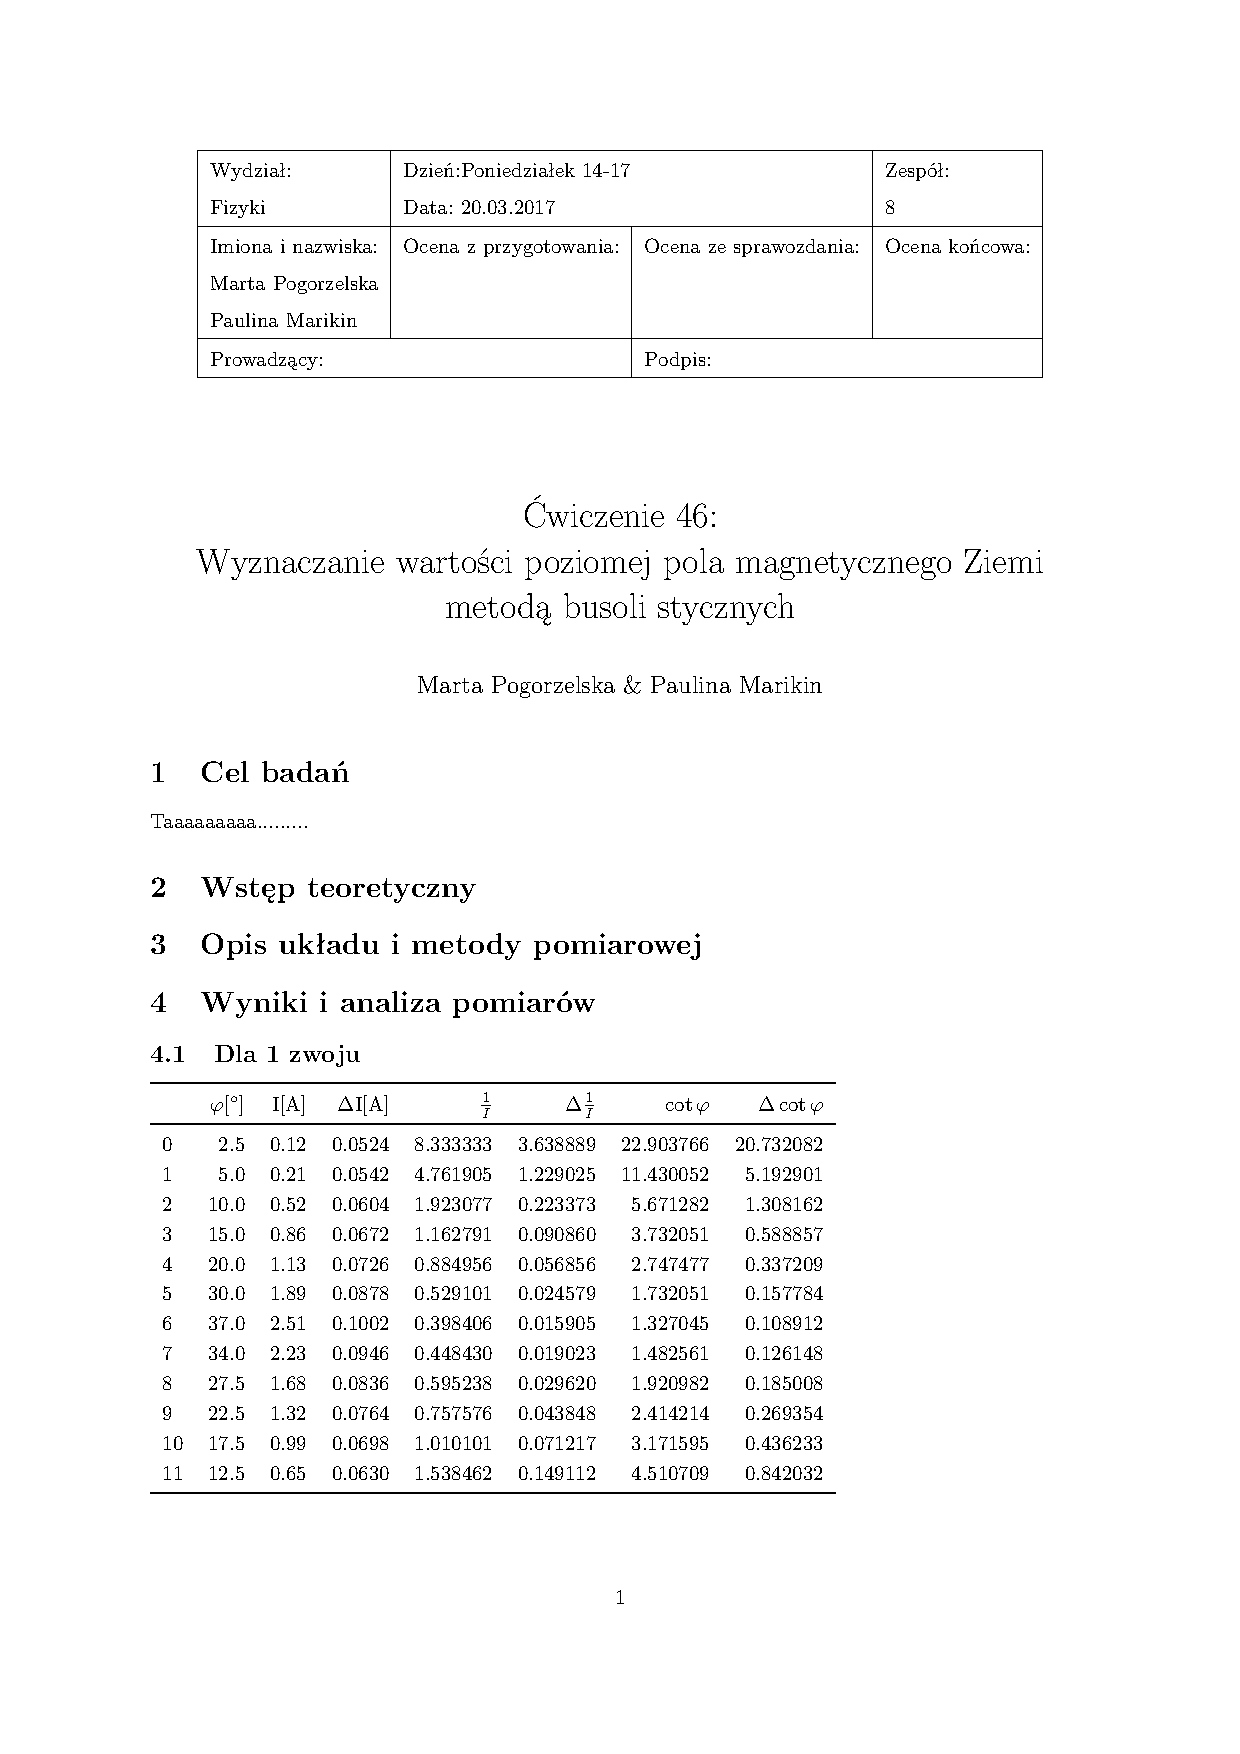
\includegraphics{./busola.png}
  \caption{Schemat busoli stycznych oraz wektory składowej poziomej natężenia ziemskiego $H_g$ i natężenia obwodu $H_o$.}
  \label{}
\end{figure}
Najpierw należało uruchomić komputer i podłączyć zasilacz do amperomierza i busoli stycznych, w taki sposób aby liczba zwojów cewki busoli wynosiła 1. Następnie włączono specjalny program na komputerze, który pokazywał obraz z kamery umieszczonej bezpośrednio nad igłą magnetyczną. Wpierw poczekano aż igła będzie w stanie równowagi i ustawiono busolę tak, by linia $0^\circ$ na kątomierzu pokrywała się z kierunkiem igły. Po ustabilizowaniu układu minimalnie podwyższono natężenie prądu w zasilaczu tak, by igła wychyliła się o pewien kąt $\varphi$. Odczytano i spisano kąt odchylenia do protokołu. Wykonano 12 pomiarów kątów wychyleń z przedziału od $0^\circ - 90^\circ$dla coraz to wyższych wartości prądu. Doświadczenie przeprowadzono analogicznie również dla 3 i 5 zwojów na cewce. W tym celu przełączono kabel między zasilaczem a cewką tak, by zwiększyć liczbę zwojów. 
\\
\\Użyte przyrządy i materiały:
\begin{itemize}
  \item busola stycznych:
    \begin{itemize}
      \item cewka pierścieniowa
      \item tarcza wraz z kątomierzem
      \item igła magnetyczna
      \item kamerka podłączona do komputera
    \end{itemize}
  \item komputer mierzący pomiary
  \item amperomierz METEX M-3650D klasy $2\%$
  \item zasilacz prądu stałego
  \item kable
\end{itemize}

\section{Wyniki i analiza pomiarów}
\subsection{Dla N = 1}
\begin{tabular}{lrrrrrrrr}
\toprule
{} &  $\varphi[^\circ]$ &  $\Delta \varphi[^\circ]$ &  I[A] &  $\Delta$I[A] &  $\frac{1}{I}$ &  $\Delta \frac{1}{I}$ &  $\cot{\varphi}$ &  $\Delta \cot{\varphi}$ \\
\midrule
0  &                2.5 &                     3.227 &  0.12 &         0.052 &          8.333 &                 3.639 &           22.904 &                  29.606 \\
1  &                5.0 &                     3.227 &  0.21 &         0.054 &          4.762 &                 1.229 &           11.430 &                   7.416 \\
2  &               10.0 &                     3.227 &  0.52 &         0.060 &          1.923 &                 0.223 &            5.671 &                   1.868 \\
11 &               12.5 &                     3.227 &  0.65 &         0.063 &          1.538 &                 0.149 &            4.511 &                   1.202 \\
3  &               15.0 &                     3.227 &  0.86 &         0.067 &          1.163 &                 0.091 &            3.732 &                   0.841 \\
10 &               17.5 &                     3.227 &  0.99 &         0.070 &          1.010 &                 0.071 &            3.172 &                   0.623 \\
4  &               20.0 &                     3.227 &  1.13 &         0.073 &          0.885 &                 0.057 &            2.747 &                   0.482 \\
9  &               22.5 &                     3.227 &  1.32 &         0.076 &          0.758 &                 0.044 &            2.414 &                   0.385 \\
8  &               27.5 &                     3.227 &  1.68 &         0.084 &          0.595 &                 0.030 &            1.921 &                   0.264 \\
5  &               30.0 &                     3.227 &  1.89 &         0.088 &          0.529 &                 0.025 &            1.732 &                   0.225 \\
7  &               34.0 &                     3.227 &  2.23 &         0.095 &          0.448 &                 0.019 &            1.483 &                   0.180 \\
6  &               37.0 &                     3.227 &  2.51 &         0.100 &          0.398 &                 0.016 &            1.327 &                   0.156 \\
\bottomrule
\end{tabular}

\\
\\Tabela nr 1: Pomiary kąta i natężenia prądu wraz z niepewnościami dla liczby zwojów N = 1.
\\
\\Parametr kierunkowy prostej $a_1$ został wyliczony, wraz z niepewnościami, przy użyciu funkcji \emph{polyfit} pakietu \emph{numpy} w Pythonie. Funkcja ta
dopasowuje prostą przy użyciu metody najmniejszych kwadratów, przyjmując dla każdego punktu wagę $\frac{1}{\text{dy}}$. Przekształcając wzór (3) dostajemy:
\begin{equation}
ctg\varphi = \frac{2RH_g}{N}\frac{1}{I}
\end{equation}
,gdzie $a_1=\frac{2RH_g}{N}$, R = 0,149 [m]

\begin{figure}[H]
  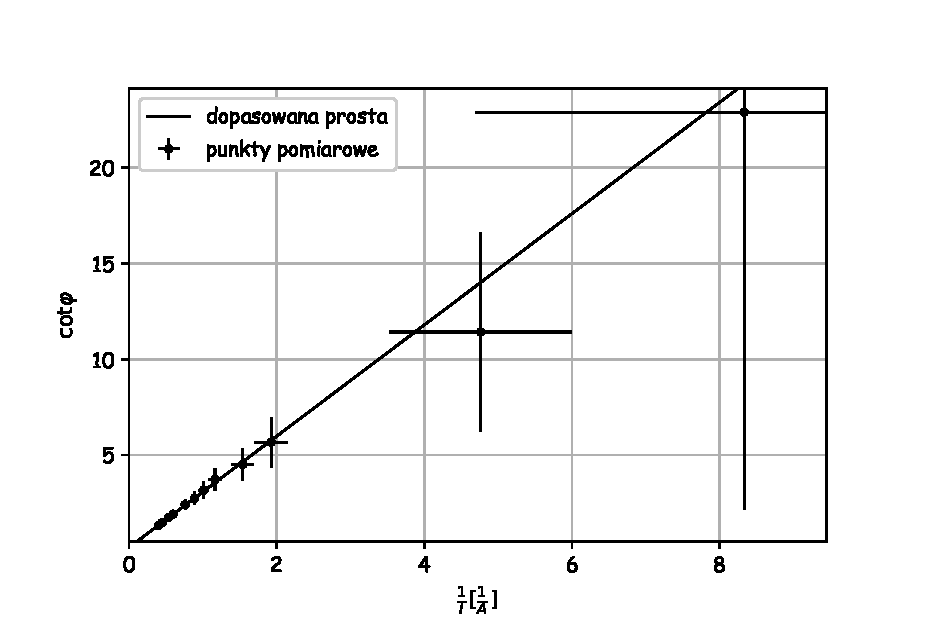
\includegraphics{./wykres_1.eps}
  \renewcommand*{\figurename}{Wykres nr} 
  \caption{Zależność ctg kąta $\varphi$ od odwrotności natężenia prądu I dla jednego zwoju.}
  \label{}
\end{figure}.
\\$a_1$ = 2.904(0.074)\\
$H_g1$ = 9.746(0.136)\\
\\Dla pozostałych obliczeń z pomiarów dla liczby zwojów 3 i 5 postępujemy analogicznie.

\subsection{Dla N = 3}
\begin{tabular}{lrrrrrrrr}
\toprule
{} &  $\varphi[^\circ]$ &  $\Delta \varphi[^\circ]$ &  I[A] &  $\Delta$I[A] &  $\frac{1}{I}$ &  $\Delta \frac{1}{I}$ &  $\cot{\varphi}$ &  $\Delta \cot{\varphi}$ \\
\midrule
0  &                2.5 &                     5.675 &  0.04 &         0.051 &         25.000 &                31.750 &           22.904 &                  52.058 \\
1  &               12.5 &                     5.675 &  0.26 &         0.055 &          3.846 &                 0.817 &            4.511 &                   2.114 \\
2  &                9.0 &                     5.675 &  0.18 &         0.054 &          5.556 &                 1.654 &            6.314 &                   4.047 \\
3  &               17.0 &                     5.675 &  0.37 &         0.057 &          2.703 &                 0.419 &            3.271 &                   1.159 \\
4  &               21.0 &                     5.675 &  0.48 &         0.060 &          2.083 &                 0.259 &            2.605 &                   0.771 \\
5  &               26.0 &                     5.675 &  0.61 &         0.062 &          1.639 &                 0.167 &            2.050 &                   0.515 \\
6  &               38.0 &                     5.675 &  0.88 &         0.068 &          1.136 &                 0.087 &            1.280 &                   0.261 \\
7  &               40.0 &                     5.675 &  1.15 &         0.073 &          0.870 &                 0.055 &            1.192 &                   0.240 \\
8  &               45.0 &                     5.675 &  1.35 &         0.077 &          0.741 &                 0.042 &            1.000 &                   0.198 \\
9  &               50.0 &                     5.675 &  1.65 &         0.083 &          0.606 &                 0.030 &            0.839 &                   0.169 \\
10 &               60.0 &                     5.675 &  2.43 &         0.099 &          0.412 &                 0.017 &            0.577 &                   0.132 \\
11 &               66.0 &                     5.675 &  3.23 &         0.115 &          0.310 &                 0.011 &            0.445 &                   0.119 \\
\bottomrule
\end{tabular}

\\
\\Tabela nr 2: Pomiary kąta i natężenia prądu wraz z niepewnościami dla liczby zwojów N = 3.

\begin{figure}[H]
  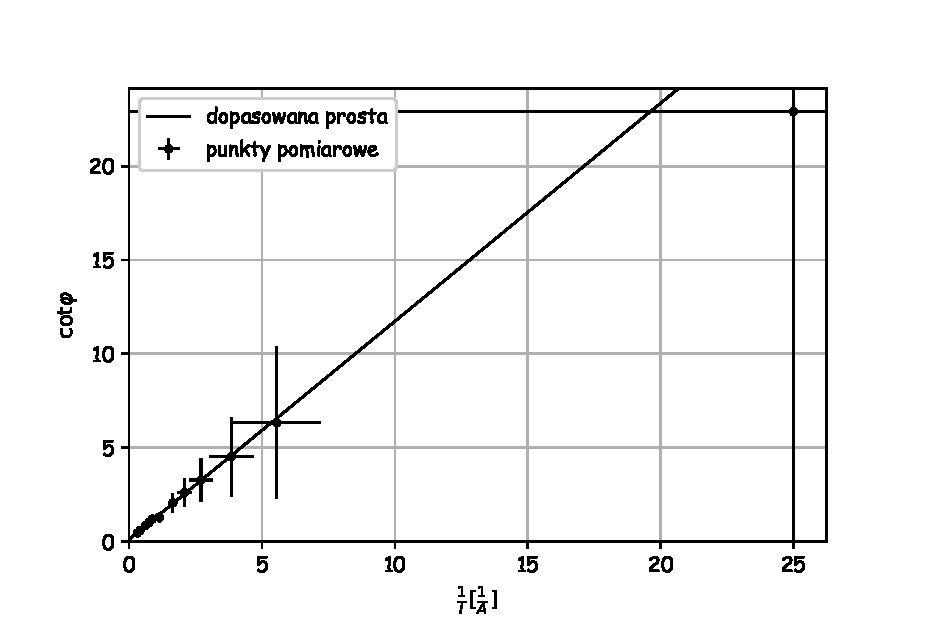
\includegraphics{./wykres_3.eps}
  \renewcommand*{\figurename}{Wykres nr} 
  \caption{Zależność ctg kąta $\varphi$ od odwrotności natężenia prądu I dla trzech zwojów.}
  \label{}
\end{figure}.
\\$a_2$ = 1.163(0.048)\\
$H_g2$ = 11.705(0.153)\\

\subsection{Dla N = 5}
\begin{tabular}{lrrrrrrrr}
\toprule
{} &  $\varphi[^\circ]$ &  $\Delta \varphi[^\circ]$ &  I[A] &  $\Delta$I[A] &  $\frac{1}{I}$ &  $\Delta \frac{1}{I}$ &  $\cot{\varphi}$ &  $\Delta \cot{\varphi}$ \\
\midrule
0  &                5.0 &                     3.23 &  0.09 &         0.052 &         11.111 &                 6.395 &           11.430 &                   7.416 \\
1  &               16.0 &                     3.23 &  0.29 &         0.056 &          3.448 &                 0.663 &            3.487 &                   0.741 \\
2  &               25.0 &                     3.23 &  0.49 &         0.060 &          2.041 &                 0.249 &            2.145 &                   0.315 \\
3  &               27.5 &                     3.23 &  0.57 &         0.061 &          1.754 &                 0.189 &            1.921 &                   0.264 \\
4  &               32.0 &                     3.23 &  0.68 &         0.064 &          1.471 &                 0.138 &            1.600 &                   0.201 \\
5  &               38.0 &                     3.23 &  0.88 &         0.068 &          1.136 &                 0.087 &            1.280 &                   0.149 \\
6  &               44.0 &                     3.23 &  1.12 &         0.072 &          0.893 &                 0.058 &            1.036 &                   0.117 \\
7  &               50.0 &                     3.23 &  1.36 &         0.077 &          0.735 &                 0.042 &            0.839 &                   0.096 \\
8  &               53.0 &                     3.23 &  1.55 &         0.081 &          0.645 &                 0.034 &            0.754 &                   0.088 \\
9  &               57.0 &                     3.23 &  1.78 &         0.086 &          0.562 &                 0.027 &            0.649 &                   0.080 \\
10 &               66.0 &                     3.23 &  2.70 &         0.104 &          0.370 &                 0.014 &            0.445 &                   0.067 \\
11 &               70.0 &                     3.23 &  3.33 &         0.117 &          0.300 &                 0.011 &            0.364 &                   0.064 \\
\bottomrule
\end{tabular}

\\
\\Tabela nr 3: Pomiary kąta i natężenia prądu wraz z niepewnościami dla liczby zwojów N = 5.

\begin{figure}[H]
  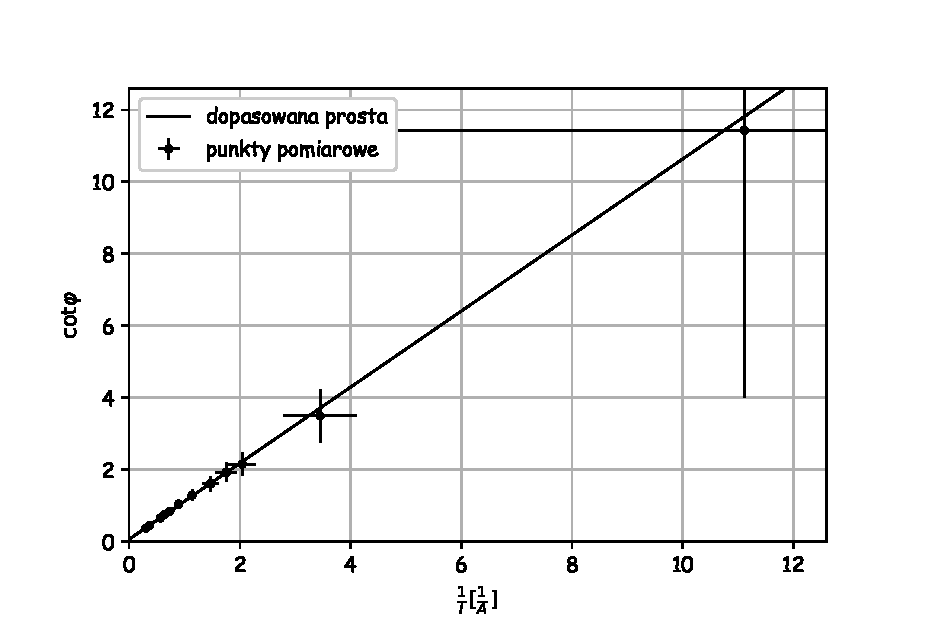
\includegraphics{./wykres_5.eps}
   \renewcommand*{\figurename}{Wykres nr} 
   \caption{Zależność ctg kąta $\varphi$ od odwrotności natężenia prądu I dla pięciu zwojów.}
  \label{}
\end{figure}.
\\$a_3$ = 1.058(0.017)\\
$H_g3$ = 17.749(0.070)\\

\section{Analiza niepewności}
Za niepewność pomiaru kąta przyjęto wartość daną wzorem:
\begin{equation}
  \Delta \varphi = \sqrt{\bigg(\frac{\text{podziałka}}{\sqrt{3}}\bigg)^2+\bigg(\frac{\text{experymentator}}{\sqrt{3}}\bigg)^2}
\end{equation}
przujmując podziałkę co $5^\circ$, i niepewność eksperymentatora równą połowie podziałki.
\\
\\Niepewności dla pomiaru prądu:
\begin{equation}
  \Delta I = I*0.02+5dgt
\end{equation}
Dla wartości potrzebnych do wyrysowania wykresu niepewności wyliczono metodą propagacji niepewności:\\
\begin{equation}
  \Delta \frac{1}{I} = \Delta I * \frac{1}{I^2}
\end{equation}
\begin{equation}
  \Delta \cot{\varphi} = \Delta \varphi * \frac{1}{\sin^2{\varphi}}
\end{equation}
Niepewność dla a uzyskano pierwiastkując zwracaną przez funkcję \emph{polyfit} kowariancję tegoż współczynnika. W celu wyznaczenia niepewności składowej pola
magnetycznego użyto %znowu
metody różniczki zupełnej:
\begin{equation}
  \Delta H_g = \Delta a * \frac{N}{2R}%Tu mogę jeszcze walnąć rozdzielczość promienia
\end{equation}
\section{Wnioski}


\end{document}
